
\documentclass[a5paper]{article}

\usepackage{amsmath, amssymb}
\usepackage{multicol}
\setlength{\columnsep}{1cm}
\usepackage[margin=0.75in]{geometry}
\usepackage{graphicx}
\graphicspath{ {../../../Images/COIT11237/} }
\usepackage[breaklinks, hidelinks]{hyperref}
\usepackage{siunitx}
\usepackage{tikz}
\usepackage{pgfplots}
\pgfplotsset{compat=newest}
\usepgfplotslibrary{external}
\usepackage{stix}
\usepackage{ragged2e}
\usepackage{enumitem}
\usepackage{polynom}

\newcommand{\sech}{\mathrm{sech}}
\newcommand{\csch}{\mathrm{csch}}
\setcounter{secnumdepth}{4}
\renewcommand\paragraph{\@startsection{paragraph}{4}{\z@}%
% display heading, like subsubsection
                                     {-3.25ex\@plus -1ex \@minus -.2ex}%
                                     {1.5ex \@plus .2ex}%
                                     {\normalfont\normalsize\bfseries}}
\sisetup{
	round-mode = places,
	round-precision = 2,
}

\date{11\textsuperscript{th} of June 2026}

\begin{document}
	\begin{titlepage}
		\centering
		{\Huge \textsc{COIT11237}\par}
		\vspace{1cm}
		{\Large \textsc{Lecture Notes}\par}
		\vspace{2.5cm}
		\vfill
		Authored by\par
		Lachlan J. W. Wyer
		\vfill
		\makeatletter
		{\large Document Start Date: \@date \par}
		\makeatother
		{\large Latest Update: \today\par}
	\end{titlepage}
	\tableofcontents
	\pagebreak

	\section{Introduction to Databases}
	\subsection{What is MySQL?:}
	Structured Query Language (SQL) is the language used to manage relational database management systems (RDBMS). It follows the CRUD principles. In that it Create, Replace, Update, \& and Deletes. SQL is used in both small \& large scale applications.
	\subsection{Databases:}
	A database (DB) can be made up of multiple tables. The conventional naming is singular. For examples, a customers' information DB would just be named customer, not customers. The table also needs a primary key (PK) as a unique identifier. This is so a singular record can be found. Tables can also be linked together through foreign keys (FK) which is just a PK in another table. When this is done, a relational database is created.
	\subsection{Problems with Spreadsheets}
	\begin{enumerate}
		\item Have redundant/wrong/out-of-date data present within the sheet. This can create conflicting copies throughout.
		\item Multiple themes per row creates modification problems
		\begin{itemize}
			\item Insertion anomalies
			\item Deletion anomalies
		\end{itemize}
	\end{enumerate}
	\subsection{Database System Components:}
	\begin{itemize}
		\item Users use forms/reports to modify data
		\item Database application converts user inputs into SQL data, which is then sent to DBMS
		\item DBMS:
		\begin{itemize}
			\item Processes the SQL
			\item Enforces the DB rules
			\item Provides concurrency, security, back-up and recovery
		\end{itemize}
		\item Database is where the data is physically stored
	\end{itemize}
	\subsection{SQL:}
	SQL is an international standard for the talking with DBs and their tables. For example:\\[1\baselineskip]
	SELECT *\\
	FROM Table.name\\
	WHERE ID = 1
	\subsection{Personal DBs:}
	These are typically just local DBs and tables stored on the system. They can be found with the localhost flags. A crucial part of local DBs is that they only support one connection at a time.
	\subsection{Commercial DBs:}
	Multiple connections with many things happening at once. Connections are usually facillitated through JAVA or C\#.

	\section{SQL Part 1}
	\subsection{Keys:}
	\subsubsection{Primary}
	When creating a table in SQL it must have a unique identifier. For example:
	\begin{center}
	\begin{tabular}{ c | c }
		EmployeeID & FirstName\\
		\hline
		1 & Lachlan \\
		2 & Paul \\
		3 & Paul
	\end{tabular}
	\end{center}
	\subsubsection{Composite}
	Sometimes a comp PK is utilized to define N:M relational tables. As long as the pair of keys is unique, the table will not break. For example:
	\begin{center}
	\begin{tabular}{ c | c }
		ProjectID & EmployeeID\\
		\hline
		1200 & 1\\
		1300 & 1\\
		1300 & 2\\
		1400 & 2
	\end{tabular}
	\end{center}
	\subsubsection{Foreign}
	These keys allow relationships between tables to form. The link must be done back to a PK in the other table. When setting a FK during the creation of the table there are two points to understand:
	\begin{enumerate}
		\item Cascade Delete: Once the original PK is deleted all rows with it as a FK
		\item Cascade Update: Same as delete, but with updating all FK rows
	\end{enumerate}
	\subsection{SELECT Clause:}
	Used to select rows of data from a table. There are only two compulsary parts to the statements. That being the column names and table name or names. To remove duplicate rows doing a SELECT DISTINCT statement will remove duplicate rows.
	\subsection{WHERE Clause:}
	Filters rows by constraining items that are in the column name. For example:\\
	SELECT EmployeeName\\
	FROM employee\\
	WHERE EmployeeID = 1\\[1\baselineskip]
	Further constraints can be added to the WHERE clause. Such as, IN, NOT, ALL, BETWEEN, IS NULL/IS NOT NULL, and LIKE. The LIKE can be defined with \% for infinite number of characters and \_ for 1 character. The \_ can be done multiple times (e.g. \_ \_ \_, but joined together like \_\_\_) for a set defined number of characters.
	\subsection{Ordering Rows:}
	Use the ORDER BY after the WHERE. Ordering can either be defined DESC or ASC, with most DBMSs having ASC as the default.
	\subsection{Having:}
	This is basically just a WHERE clause for grouped functions. When in a statement with WHERE clauses, the WHERE clause is applied before the HAVING.
	\subsection{Subqueries:}
	SELECT * \\
	FROM table1\\
	WHERE column IN (subquery)

	\section{SQL - Part 2}
	\subsection{Joins of Tables:}
	There a number of different types of joins. Joins can be used consecutaley to have multiple different tables joined together. The column used to join the table must be the same in each one. For example, an INNER JOIN is similary to,\\
	FROM table1 as T1 \\
	INNER JOIN table2 as T2 ON T1.id = T2.id
	\begin{center}
		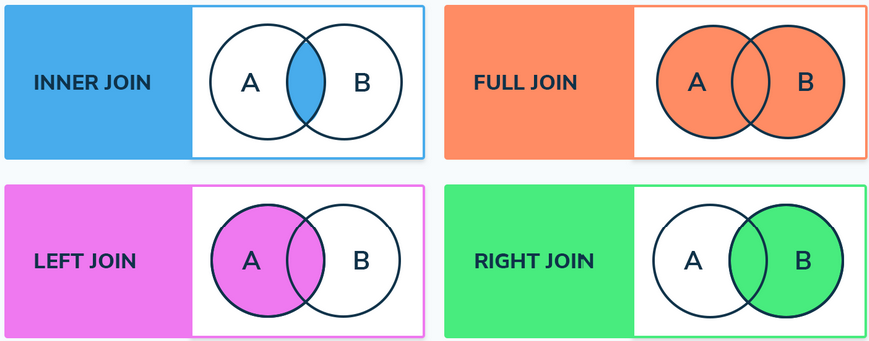
\includegraphics[scale=0.75]{joins.png}
	\end{center}
	\subsection{Union:}
	These are used to completely join two tables together. This is similar to a full join. For example,\\
	(SELECT * FROM table1)\\
	UNION\\
	(SELECT * FROM table2)
	\subsection{Modifying Data:}
	Used when updating/deleting a row of data. As well as creating or dropping a table.

	\section{ER Diagrams}
	A formal presentation of user requirements. They help refine the requirements before a database is created.
	\subsection{Purpose:}
	Help visualizes the relationships between the tables.
	\begin{itemize}
		\item What thing's are stored within the DB?
		\item What do we want to know about these things?
		\item Are there any relationships between the tables?
		\item Are there any constraints in the DB?
	\end{itemize}
	To summmarize ER diagrams help define the entire requirements of the DB system.
	\subsection{Database Definition:}
	A DB contains a definition of its data. Specifically, the meta-data is the specific data describing the structure of DBs data. These include the datatype (INT, DATE, CHAR \& VARCHAR), uniqueness, auto-increment, and length.
	\subsection{Entity Representation:}
	Simply, name it an entity if it is more than just a name of something. I.E. Has non-key attributes or relationships with multiple entities.
	\subsection{Identifier:}
	Entity instances have an identifier. These are attributes that are unique (E.g. PKs) across all instances. Sometimes a composite of 2 or more identifiers to make a unique key.
	\subsection{Relationships:}
	Minimum cardinality: The minimum number of instances that must be involved with an instance.\\
	Maximum cardinality: The maximum number of instances that a relationships can have.
	\begin{center}
		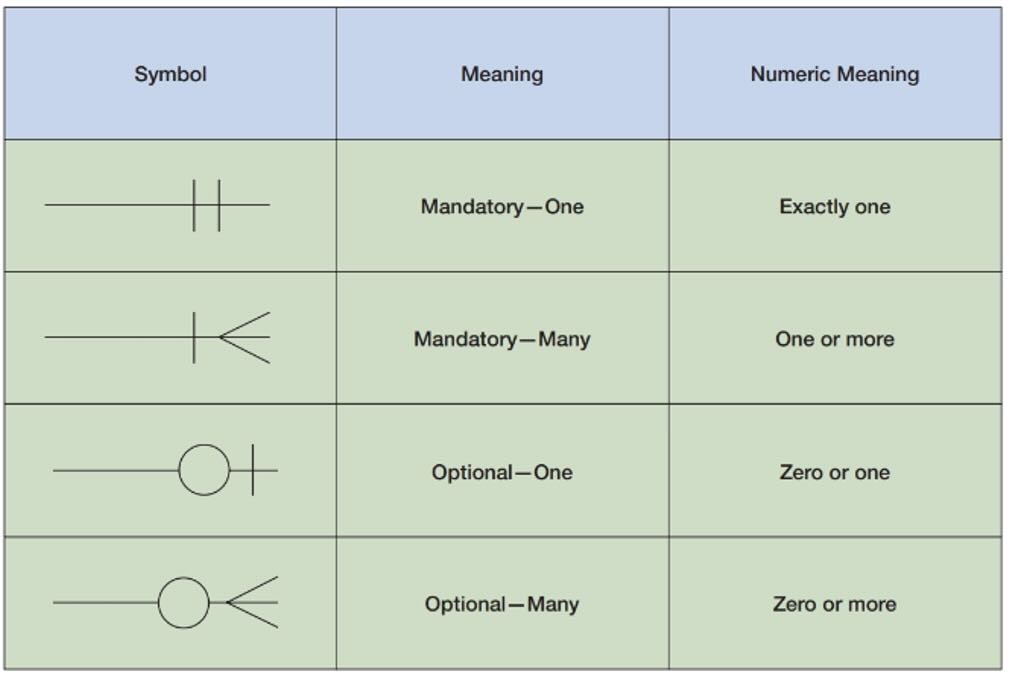
\includegraphics[scale=0.35]{cardinality-symbols.png}
	\end{center}
	When drawing these, if connected by a dashed line, both entities are independent of each other.
	\subsection{Modelling ERDs:}
	\begin{enumerate}
		\item Write out all entities
		\item Display relationships and state any assumptions made with them
		\item Check if any extra modelling is required
	\end{enumerate}
	\subsection{Weak Entity:}
	A WE is an entity that cannot exist in a DB without another entity also existing. That being if the strong entity is removed, the weak one must also be removed.
	\begin{center}
		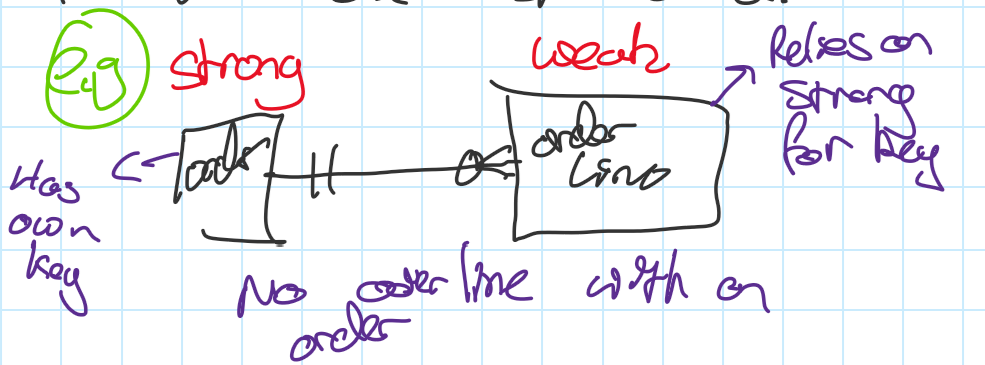
\includegraphics[scale=0.5]{weak-entity.png}
	\end{center}
	\subsubsection{Id-dependent}
	This relies on its parent entity for its identifier. They usually have composite identifiers within the DB. Represented through a solid line.
	\subsubsection{Non-Identifying}
	Does not rely on its parent entity for its unique identification. Illustrated by a dashed line to represent the lack of dependency.

	\section{ER Digrams - 2}
	\subsection{Associative Entities:}
	It is best practice to avoid N:M relationships between entities. To do this a third entity is made with 2 1:N relationships. This entity is then an id-dependent on both sides.
	\subsection{Subtype:}
	A type of entity that inherts the attributes and relationships of the more general super-type. Further specifc attributes can be added to the sub-type entities. Sub-type entities reduce reduncy by placing common atrributes in a super-type, whilst also keeping singular attributes in the sub-type.
	\begin{center}
		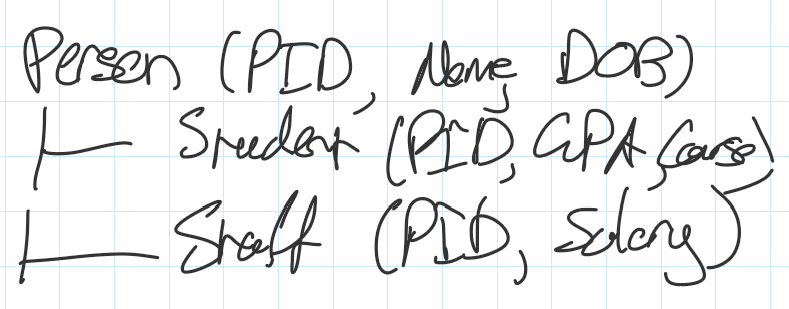
\includegraphics[scale=0.75]{sub-type-entity.png}
	\end{center}
	\subsection{Notation:}
	Exclusive is related to atmost one sub-type.
	\begin{center}
		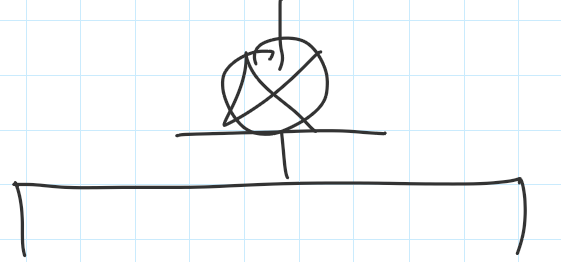
\includegraphics[scale=0.75]{exclusive-notation.png}
	\end{center}
	Inclusive is where a super-type can be related to more than 1 sub-type.
	\begin{center}
		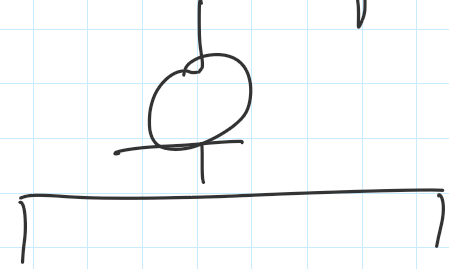
\includegraphics[scale=0.75]{inclusive-notation.png}
	\end{center}
	Sub-type entities are not suitable when:
	\begin{itemize}
		\item Categories change frequently
		\item The difference is in a represented value not in its attributes
		\item Individuals move between categories over time
	\end{itemize}
	\subsection{Recursive Relationships:}
	When a FK links too the PK within the same table. For example, an employee is supervised by a manager, who in turn an employee of the company.

	\section{Normalization}
	\subsection{Data Redundancy:}
	List and spreadsheets store excess amount of redundant data. This can cause modification anomalies craeting conflicting copies/records in the table. They also have multiple themes per row. Where deletaion anomalies, delete everything within that record, and insertion anomalies, where blank cell are created when data is inserted.
	\subsection{Relational DBs:}
	Relational DBs split the spreadsheet into smaller tables that are linked through keys. They are more work to maintain up-front, but solves the problems associated with the spreadsheets.
	\subsection{Relational Checklists:}
	All following conditions must be met to make a spreadsheet a relational DB.
	\begin{center}
		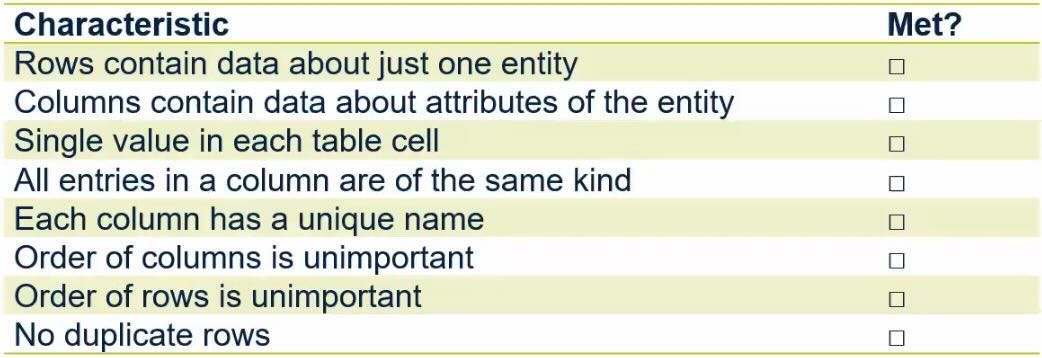
\includegraphics[scale=0.35]{relational-checklist.png}
	\end{center}
	\subsection{Candidate Keys:}
	Candidate keys are a unique set of keys that identify a single record. All these keys are capable of becoming a PK.
	\subsection{Primary Keys:}
	Notation is used to declare a relation. These include underlining \underline{PKs} and italicized \textit{FKs}. For exmaple,
	\begin{center}
		TableName(\underline{PK}, Col1, Col2, \textit{Col3})
	\end{center}
	\subsection{Boyce-Codd Normal Form:}
	BCNF is based on a concept that an attribute determines another set of attributes. If nothing determines an attribute, a unique key is added to the system. This is known as a surrogate key.
	\subsubsection{Referential Integrity:}
	For tables to satisfy it, every FK value must match  a PK value in another table.
	\subsubsection{NULL Values:}
	It is better to aviod having NULL values present within DB. This is because the specified value in the row and column is ambiguous.
	\subsubsection{Functional Dependancy:}
	Are when an attribute determines all other attribute. The main example for this is when a PK determines all values within a table.
	\subsection{BCNF:}
	The BCNF is a form of normalisation:
	\begin{itemize}
		\item Break up tables to remove anomalies
		\item Stream line data
		\item Stops replication of data points
	\end{itemize}

	\section{Database Design}
	\subsection{ER Diagrams to Tables:}
	Defining the data types present. This determines what will be placed within the column, INT or VARCHAR. Each column also needs to be assigned one specific data type. Further points can be NULL level status, whether a value can be a NULL value or whether a default value should be assigned. In addition the data in the column can also be constrained to a specifc type. E.g. a minimum birth year of 1800.\\
	Each entity within an ERD should have its own table created.
	\subsection{Constraints:}
	Unique constraints is similar to a PK, in that each value must be unique to each other within that column. Columns that can have this are usernames or phone numbers. An advantage of this is that the table maintains an idex. Making the sorting of unique data faster.
	\subsubsection{Checks}
	Checks force values to be within a user defined range or values. If multiple check clauses are used, the standardised way it to have seperate check statements. A check can also reference multiple columns.
	\subsection{Referential Integrity:}
	The FK needs to match PK in the parent table. When something is modified in the parent table, the FK needs to also be modified in the same way. For example, determining if when the FK in parent table is deleted do all rows with FK need to also be deleted.
	\subsection{Overall Steps:}
	\begin{enumerate}
		\item Create a table for each entity
		\item Identify the PK
		\item Identify data types
		\item Verify Normalisation
		\item Identify id-dependent/id-independent weak entity relatioships
		\item Create relatioships using FKs
	\end{enumerate}

	\section{Database Administration - Part 1}
	\subsection{DB Processing Environments:}
	\begin{center}
		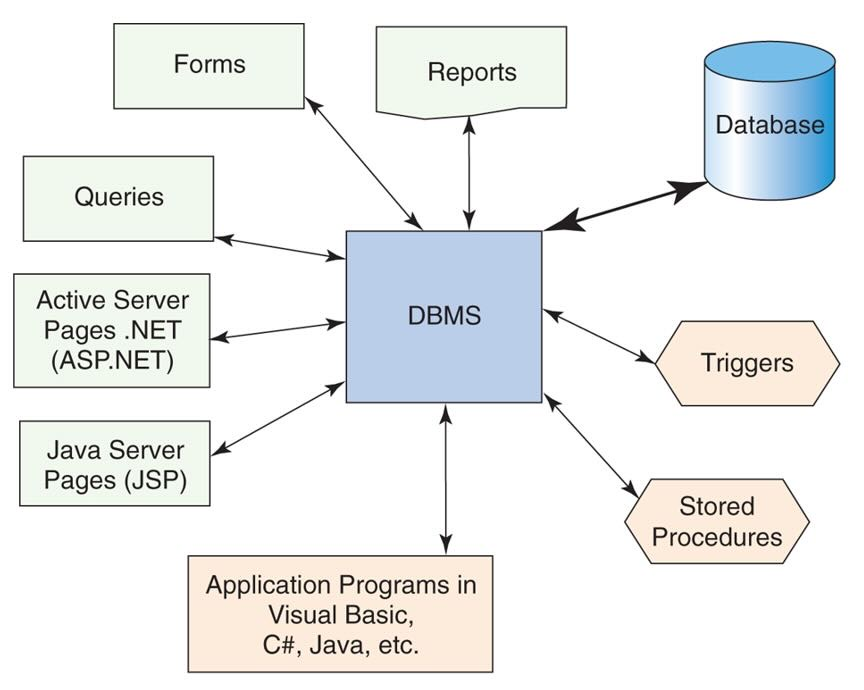
\includegraphics[scale=0.4]{db-processing-environment.png}
	\end{center}
	This is way of interacting with the DBMS from a user perspective. Convurrency is when multiple users are accessing and performing CRUD operations at once.
	\subsection{Transactions:}
	Some statements within SQL should be done in conjuction with another and never alone. If the entire query is not completed sucessfully it fails and the transaction is rolled back. For example:\\
	Stock Transfer\\
	UPDATE stock\\
	SET Qty=Qty+5\\
	WHERE Location = 'Warehouse'
	\subsection{ACID Transactions:}
	\begin{itemize}
		\item Atomic - Everything in the transaction will COMMIT or nothing will
		\item Consistent - Database is consistent before and after the tractions
		\item Isolated - The actions of one transaction does not affect another
		\item Durable - All changes are perments (saved to non-volatile storage)
	\end{itemize}
	\subsection{Concurrency Control:}
	Concurrency is needed in operations where multiple users are doing transactions on the same data. For this the accesibility scale is utilized.
	\subsubsection{Extreme Inaccessibility}
	\begin{itemize}
		\item Data is inaccessable once a user updates
		\item Data updated is not available until the transaction commits
		\item Only one person can see data at a time
	\end{itemize}
	\subsubsection{Extreme Accessibility}
	\begin{itemize}
		\item Data is always radable
		\item Even when locked for updates
	\end{itemize}
	Balancing interdependcy (Changes required by one user impact another) and record retention (How long old data is accessible).
	\subsubsection{The Lost Update Problem}
	The update is overwritten by another transaction. As the old value is read and the new value is written over.
	\begin{center}
		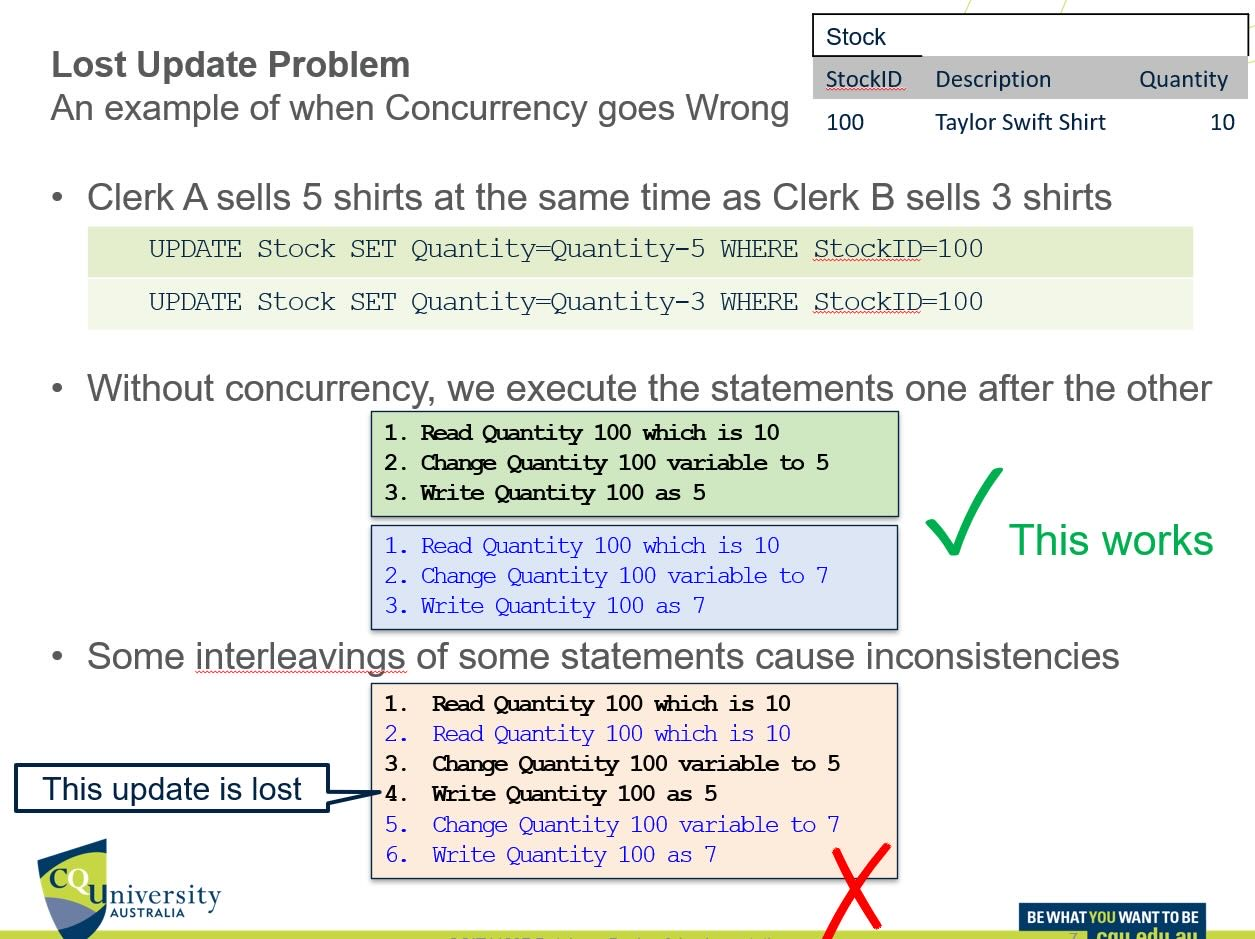
\includegraphics[scale=0.3]{lost-update.png}
	\end{center}
	\subsubsection{Dirty Reads}
	Dirty reads occur if the DBMS allow uncommitted updates as committed.
	\begin{center}
		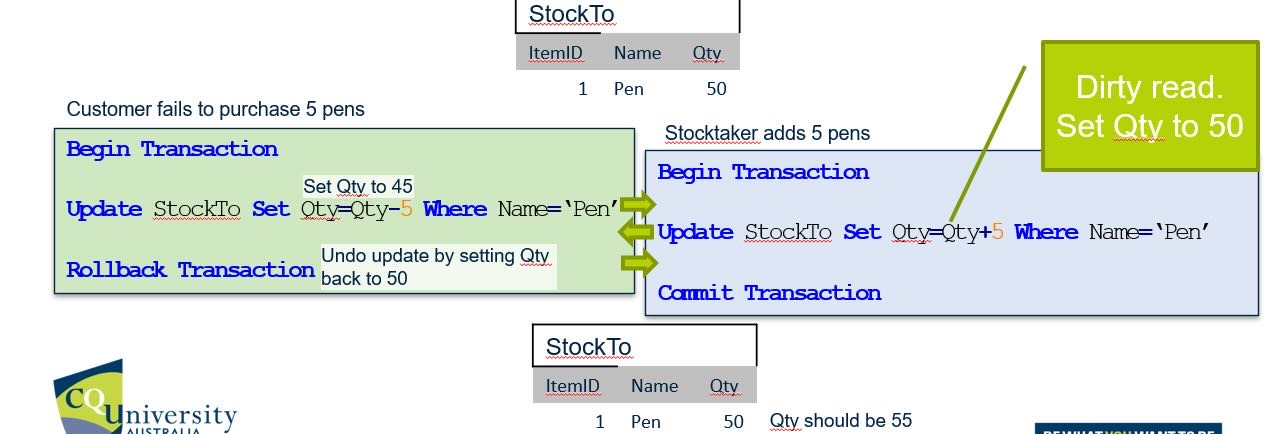
\includegraphics[scale=0.3]{dirty-reads.png}
	\end{center}
	\subsubsection{Non-repeatable Reads}
	Allow reading of committed changes during a repeating transaction.
	\begin{center}
		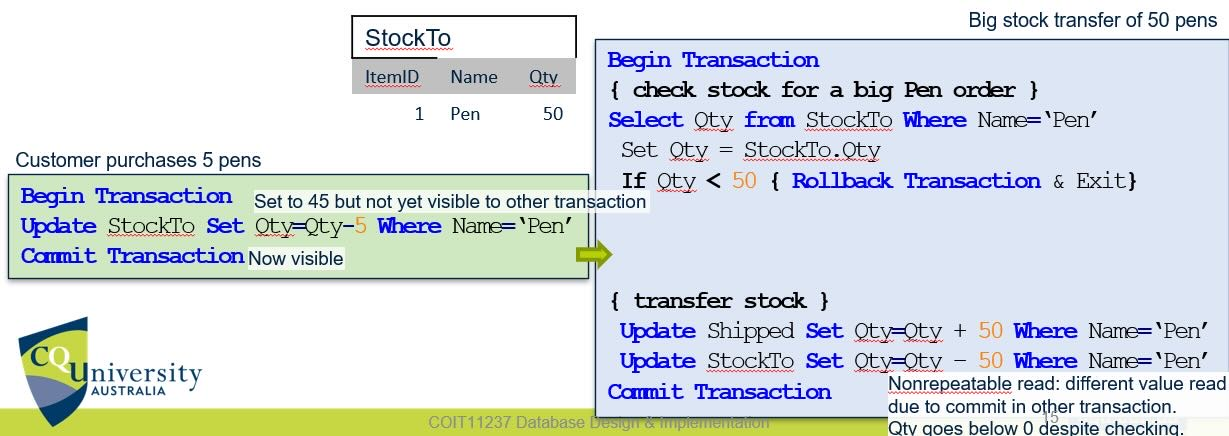
\includegraphics[scale=0.3]{non-repeatable-reads.png}
	\end{center}
	\subsubsection{Phantom Reads}
	See inserted reads partway through a transaction.
	\begin{center}
		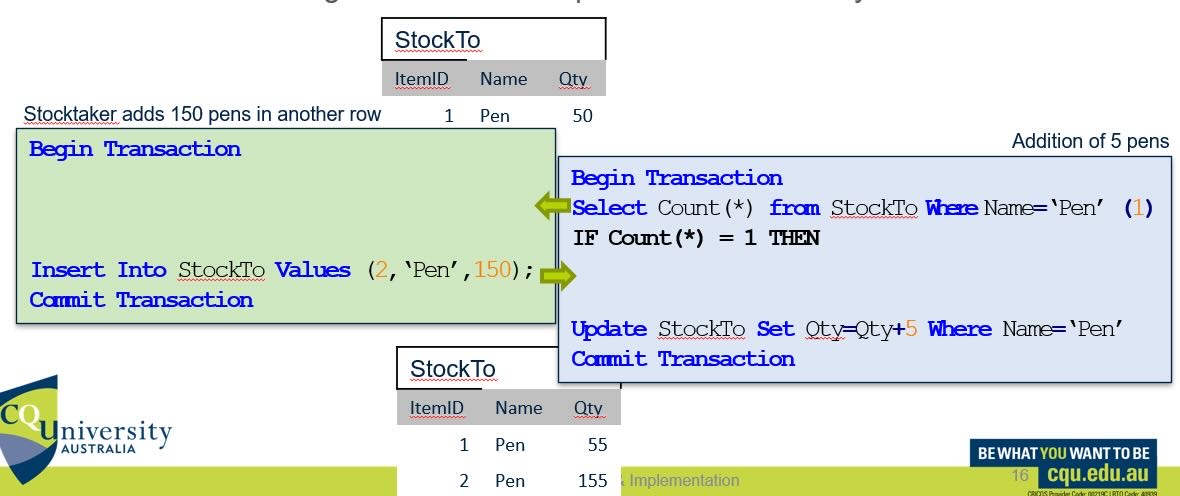
\includegraphics[scale=0.3]{phantom-read.png}
	\end{center}
	\subsection{Data Read Problems Overview:}
	\begin{center}
		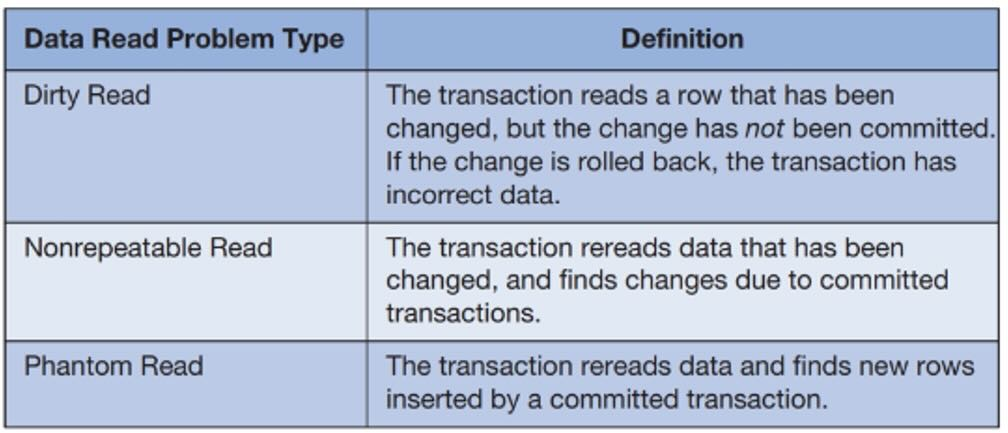
\includegraphics[scale=0.25]{data-read-problems.png}
	\end{center}
	\subsection{Resource Locks:}
	Locks disallow reading and writing to a dataset whilst in place. A client must wait until a lock is released to perform the transaction. Explicit Locks are issued by the SQL developer for their specific application. Implicit locks are isssued by the DBMS and developers do not need to worry. For these types of locks to work effectively, everything must be synchronised to a serial order. This slows down transcation timing but everything is correct with not concurrency errors.
	\subsection{Two-Phase Locking:}
	Transactions are allowed to obtain locks but once the first lock is released, no new locks can be assigned. When obtaining locks this is known as the growing phase, and the releasing of locks is known as the shrinking phase. 2PL cannot prevent the phantom reads occuring.
	\subsection{Deadlock:}
	2PL transactions can suffer from something called deadlock. This occures when two transactions wait indefinitely for each other to release their lock. Almost every DBMS has algorithms in place to detect and prevent deadlock. When a deadlock occures, roll-back of one of the transactions to remove its changes occurs. Locking strategies can include:
	\begin{itemize}
		\item Optimistic
		\item Pessimistic
	\end{itemize}
	\subsubsection{Optimistic}
	Based on the assumption that no conflict will occur.
	\begin{enumerate}
		\item Data is read
		\item Data is processed
		\item Updates issued
		\item Check to see if a conflict occured
		\begin{itemize}
			\item No conflict - Finish the transaction
			\item Conflict - Repeat until processed without conflict (Locks can be placed)
		\end{itemize}
	\end{enumerate}
	\subsubsection{Pessimistic}
	Uses the assumption that in all transactions a conflict will occur.
	\begin{enumerate}
		\item Locks issued
		\item The transaction is processed
		\item Locks released
	\end{enumerate}
	Optimistic locking is generally faster as locks are held for less time. However transactions might need to be repeated numerous times to not have errors. Pessimistic locking is used when the risk of conflict is high or systems are always connected to the DBMS.
	\subsection{Transaction Isolation Levels:}
	\begin{enumerate}
		\setcounter{enumi}{-1}
		\item Read Uncommitted
			\begin{itemize}
				\item Lowest isolation level
				\item Data inconsistency and integrity issues
				\item Allows dirty reads, non-repeatable reads and phantom reads
			\end{itemize}
		\item Read Committed
			\begin{itemize}
				\item Only read committed data
				\item Only stops dirty reads
				\item Allows non-repeatable reads and phantom reads
			\end{itemize}
		\item Repeatable Read
			\begin{itemize}
				\item Locking rows that are read or modified until completion
				\item Stops dirty reads and non-repeatable reads
				\item Does not prevent phantom reads
			\end{itemize}
		\item Serialized
			\begin{itemize}
				\item Highest isolation level
				\item Prevents all concurrency issues
				\item Slowest
			\end{itemize}
	\end{enumerate}
	\begin{center}
		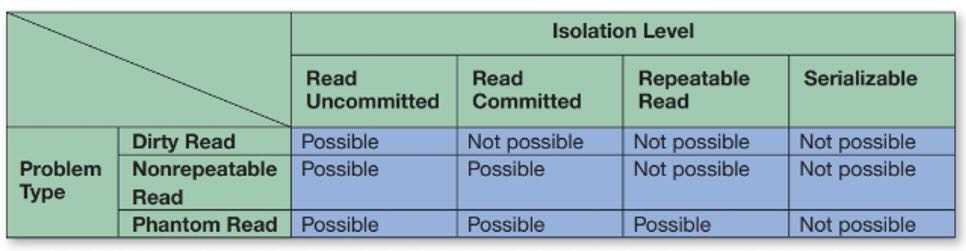
\includegraphics[scale=0.3]{isolation-levels.png}
	\end{center}
	In theory there is no matching between 2PL and isolation levels.\\
	Within MySQL, it defaults to level 2.

	\section{Database Admin - Part 2}
	\subsection{DB Security:}
	\begin{itemize}
		\item Authentication: Who are you?
		\item Authorization: Are you allowed to do that?
	\end{itemize}
	\subsection{DB Security Guidelines:}
	\begin{itemize}
		\item Run the DBMS behind firewalls.
		\item Keep everything updated with latest security patches.
		\item Limit DBMS functionality to smallest amount. This is the principle of least privilge.
		\item Protect the computer running the DBMS
			\begin{itemize}
				\item Anti-virun software
				\item Locks
				\item Access
				\item High Availability
			\end{itemize}
		\item Manage Accounts and Passwords
	\end{itemize}
	\subsection{DB Failures:}
	Common failure points include:
	\begin{itemize}
		\item Hardware failures
		\item Programming bugs
		\item Human error/mistakes
		\item Malicious actions
	\end{itemize}
	As they are very hard to prevent completely, recovery procedures are essential.
	\subsection{Recovery via Reprocessing:}
	\begin{enumerate}
		\item Start from an earlier back-up
		\item Reapply all transactions that happened after that back-up
	\end{enumerate}
	Reprocessing is:
	\begin{itemize}
		\item Costly due to re-entering all data
		\item Risky due to increased amount of human-error, records of all transactions not being there, and some operations producing different results when re-run.
	\end{itemize}
	\subsection{Recovery via Rollback:}
	Simply just an undo button. To undo a transaction, the log must contain a copy of the database before any change. This is known as a before image. A transaction can be undone by applying before images of changes to the DB.
	\subsubsection{Rollforward}
	Rollforward is the opposite of a rollback. An older state uses after images of the DB to re-apply transactions.
	\subsection{Database Administrator Responsibilities:}
	\begin{itemize}
		\item Service system\\A system to gather, record and prioritise user reported problems.
		\item Change request process - change Management, create and manage processees for controlling DB config;
			\begin{itemize}
				\item Procedure for recording change request
				\item Conducting user and developer reviews of such request
				\item Creating projects and tasks
			\end{itemize}
		\item Documentation
			\begin{itemize}
				\item Ensure documentationis maintained
				\item Database structure
				\item Concurrency control
				\item Security
				\item Back-up and recovery
				\item Applications utilized
			\end{itemize}
	\end{itemize}
	\subsection{Data Validation:}
	Ensures data within a certain range of values. Keep data consistency within the definition. The main types that SQL uses is CHECK, UNIQUE, and NOT NULL.
	\subsubsection{"CHECK" Constraint}
	\begin{itemize}
		\item Limitation are used at a DB Level
		\item Validates data
		\item Evaluated on INSERT, UPDATE, REPLACE and LOAD DATA elements
	\end{itemize}
	An error is raised if a constraint evaulation goes FALSE.
	\subsection{MySQL Views:}
	A view can be treated as a virtual table consisting of only columns and rows specified in a SELECT statement. For example:\\
	CREATE VIEW view\_name AS\\
	\indent\indent SELECT column\_name\\
	\indent\indent FROM table\_name\\
	\indent\indent WHERE column\_name = "Hello World!";\\[1\baselineskip]
	SELECT * FROM view\_name\\[1\baselineskip]
	A view is a subset of a database that can be saved. The view itself does not store any data, but reflects the most current data in base table. This is really good for complex queries.
	\subsection{View Advantages:}
	\begin{itemize}
		\item Can limit the exposure of tables externals entities
		\item A view can restrict acess to seeing columns in the table
		\item It can simply queries by hiding complex retieval operations
		\item With restrictions views can update tables
	\end{itemize}
	\subsection{Stored Programs:}
	There are 4 main types:
	\begin{enumerate}
		\item Stored procedure - Can be called from anything that has acess to the DB
		\item Stored function - Called from SQL statement and returns a value
		\item Trigger - Is executed in responce to an INSERT/UPDATE/DELETE stat\-ements on a specific table
	\item Event - Is executed at a scheduled time
	\end{enumerate}
	\subsubsection{Stored Procedures}
	Calling a stored procedure without parameters
	\begin{center}
		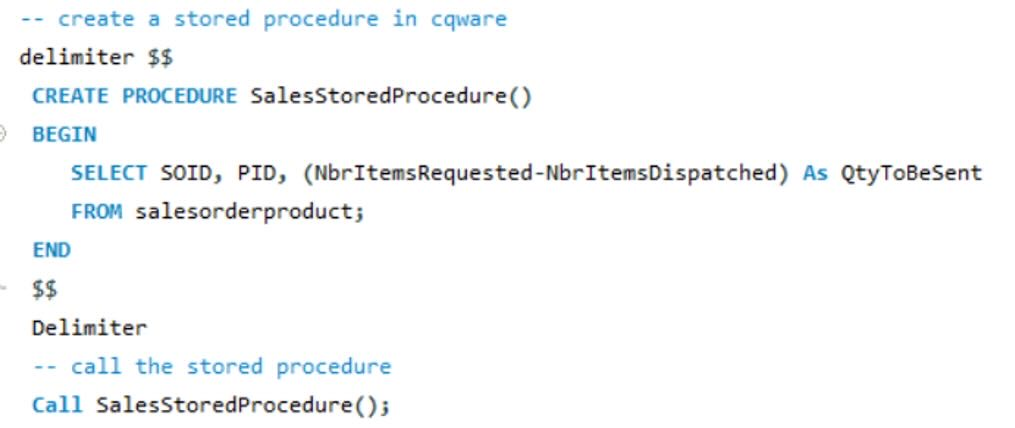
\includegraphics[scale=0.3]{stored-no-parameters.png}
	\end{center}
	A script calling parameters has some items to follow:
	\begin{itemize}
		\item IN parameters:
			\begin{itemize}
				\item IN is the default mode
				\item The program has to pass an argument to the procedure
			\end{itemize}
		\item OUT parameters:
			\begin{itemize}
				\item The value here can be charged inside the procedure and a new value\\passed back to the calling program
			\end{itemize}
	\end{itemize}
	\begin{center}
		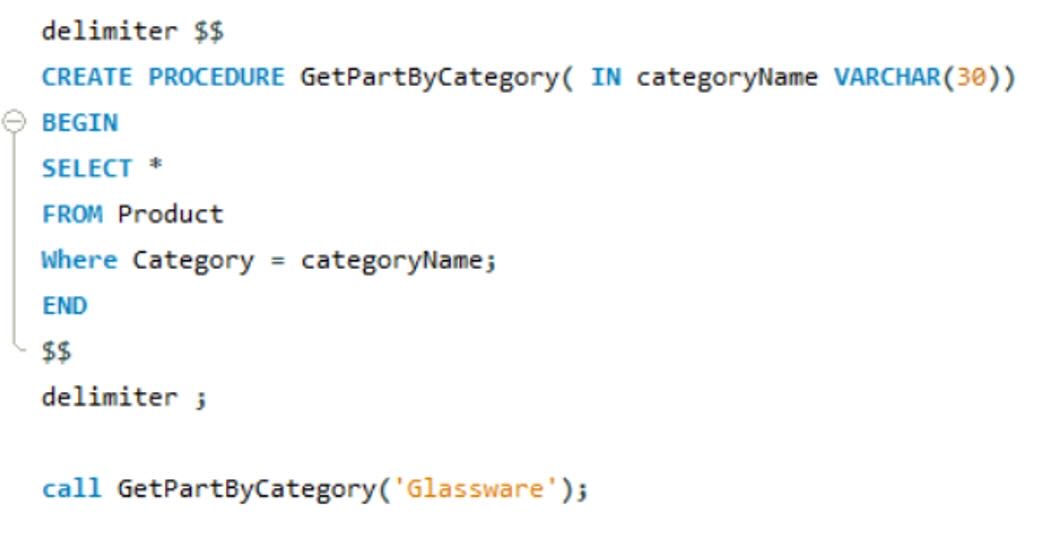
\includegraphics[scale=0.3]{stored-parameters.png}
	\end{center}
	\subsubsection{Triggers}
	A trigger is a special type of stored procedure that is used when a condition occurs BEFORE/AFTER/INSTEAD OF the transaction. Triggers provide a powerful way to enforce data consistency, log changes, ensure referential integrity and implement business rules.

	\section{Business Integration Systems}
	\subsection{Transaction Systems:}
	These are processing systems that also support day-2-day routine transactions. Key features include:
	\begin{itemize}
		\item Support normal business activities
		\item Real-time
		\item Ensure all transactions are recorded
	\end{itemize}
	\subsection{BI Systems:}
	Helps organizations use data to understand what has happened.
	\begin{itemize}
		\item Provide reports
		\item Support analysis of data
		\item Identification of patterns
		\item Predict future trends
		\item Control business direction
	\end{itemize}
	\subsection{Data Mining:}
	This is the automated discovery of patterns with large datasets. These includes clustering, association detection, and statistical analysis.
	\subsection{Integration of Datasets:}
	There are two main options:
	\begin{enumerate}
		\item Connect seperate operational databases, which is often very costly
		\item Data warehousing
			\begin{itemize}
				\item Extract from operational DBs into a new DB
				\item Reduces disruption from the day 2 day operations
			\end{itemize}
	\end{enumerate}
	\subsection{ETL Data Transformation:}
	Used when operational DB needs to be cleaned before it goes into the warehouse. It is during the ETL process in which descions above data integrity problems are made.
	\subsection{Data Mart:}
	A collection of data that is smaller than a data warehouse. This is because it addresses a specific functional areas of the business.
	\subsection{DB Application in a Business:}
	OnLine Transaction Processing (OLTP):
	\begin{itemize}
		\item Process an order
		\item Calculate sales
		\item Operational systems
		\item Using a DB to run a business
	\end{itemize}
	OnLine Analytical Processing (OLAP):
	\begin{itemize}
		\item Highest selling products
		\item Report systems
		\item Using the DB to make good business descions
	\end{itemize}
	\subsection{Distributed DB Processing:}
	Spreading the load and storage amongst several database severs.\\
	Partioned - Breaking the DB into pieces\\
	Replicated - Storing copies on multiple systems
	\subsection{Big Data:}
	DB involves large and complex datasets. These cannot be easily processed using traditional DB systems. These is no set definiton what Big Data is. However characteristics include; volume, velocity, variety, veracity.
	\subsection{Non-relational DBs:}
	Object oriented DBs have complex data structures and works well with OO programming languages.
	\subsubsection{NoSQL DB:}
	4 major types of NoSQL are:
	\begin{itemize}
		\item Key-value: Dynamo, Redis
		\item Document: CouchDB, MangoDB
		\item Column Family: Apache Cassandra
		\item Graph: Allegrograph, Titan
	\end{itemize}
	\paragraph{Advantages}
	\begin{itemize}
		\item Scalability
		\item Simplicity
		\item Less code
		\item Easy maintainence
		\item Low latency
		\item Fast write speed
	\end{itemize}
	\paragraph{Disadvantages}
	\begin{itemize}
		\item Less used
		\item Less consistent (No ACID)
		\item Less support (smaller technical community)
		\item No common language
		\item Difficult to understand data structures
	\end{itemize}
	
	\section{Cloud Systems}
	\subsection{What is Cloud Computing?:}
	It is computing technology that a user rents/leases a service/product over the internet from a service provider. Said service is usually provided by an IT giant. For example,
	\begin{itemize}
		\item Microsoft -> Azure
		\item Amazon -> AWS
		\item Alphabet -> Google Compute
	\end{itemize}
	The main features of cloud computing are:
	\begin{itemize}
		\item Remote hosting - Nothing is local
		\item Ubiquitous - Anywhere, Anytime
		\item Commodified - Pay as you go
	\end{itemize}
	\subsection{Cloud Service Models:}
	\subsubsection{Software as a Service (SaaS)}
	The SaaS model allows the use of applications as a service to end users. SaaS is a software delivery method that provides multi-tenant access to web-based functions. The bill based on usage, with a highly scaleable architecture.
	\subsubsection{Platform as a Service (PaaS)}
	PaaS provides the runtime environment for applications and development tools. Applications must be developed with a particular platform in mind.
	\subsubsection{Infrastructure as a Service (IaaS)}
	IaaS is the delivery of infrastructure as an on demand scalable service. IaaS provides access to fundamental compute resourse. E.g. HDD, SSD, CPU, GPU, and RAM.
	\subsection{Cloud Computing:}
	\subsubsection{Advantages}
	\begin{itemize}
		\item Lower local computer costs
		\item Improved performance
		\item Reduced initial costs and instant software access
		\item Scalability, easy upgrades
	\end{itemize}
	\subsubsection{Disadvantages}
	\begin{itemize}
		\item Requires constant, high-speed internet access
		\item Stored data will be lost once payments cease
		\item No digital soverignty
	\end{itemize}
	\subsection{DB Cyber Attcks:}
	As more businesses move online, an increased demand for cybersecurity is required. The most attack vector is JS and SQL injections. To defend against specifically SQL injections:
	\begin{itemize}
		\item Sanatize all data inputs
		\item Validate inputs or give no choice
		\item Use parametrized queries
		\item Use properly stored procedures
	\end{itemize}
\end{document}
